\typeout{NT FILE chapter2.tex}
\chapter{Theoretical Context} \label{lit_review}

All the necessary scientific concepts and ideas will be discussed in this section to provide the reader with a theoretical context of the task at hand.

\section{Permafrost and its degradation}  \label{perma_intro}
\paragraph{}
Permafrost is characterised as frozen ground that has a temperature colder than 0 degrees C continuously for 2 or more years (\cite{everdingen_multi-language_1998}).
% Regions can be classified according to the percentage of permafrost present in the area: continuous, discontinuous, boundary. 

As the Arctic has warmed twice as fast as the globe on average, \gls{a.k.a.} Arctic amplification (\cite{climatechangefur}) the consequences of global warming are disproportionally felt in the Arctic. 

In the Northern Hemisphere, huge amounts of soil organic carbon are trapped in permafrost soils. Any change in boundary conditions that causes the ground to warm will result in the thaw of permafrost. These abrupt thaw processes will expose previously frozen soil organic matter, causing it to undergo microbial degradation, and release GHGs e.g. methane and carbon dioxide as a result.

The thaw of permafrost (degradation) can not only lead to damage to roads and other man-made infrastructures but also lead to the release of said trapped GHGs which consequently could contribute further to global warming and even more permafrost degradation (\cite{MURTON2021857}) as it warms and thaws at a faster rate, creating a vicious cycle of global warming.

This could further exacerbate Arctic amplification, therefore it is imperative to monitor and predict the volume of GHGs released into the atmosphere due to the abrupt thaw of permafrost.

\subsection{Thermokarst landforms}  \label{thermokarst_intro}
\paragraph{}
The extent of permafrost and its degradation is difficult to measure and historically requires extensive and costly investigation. A way to attempt this is to look for evidence of the formation of thermokarst landforms such as those depicted in Figure \ref{fig_thermokrast} which cause visible geological changes in close range of abrupt thaw locations.

Thermokarst is the sinking of the ground's surface due to thawing of the ground (permafrost degradation). There are many examples of thermokarst landforms, amongst the most common and fast-changing are lakes and ponds (\cite{thawpic}).

In Figure \ref{fig_thermokrast}, identified by label number 10, we can also see another relevant example, \gls{RTS}, this paper will focus on the identification of this thermokarst feature in an attempt to capture some extent of permafrost degradation in the Arctic. The next sub-section will describe \gls{RTS}s further.

    \begin{figure}[hbt!]
        \centering
        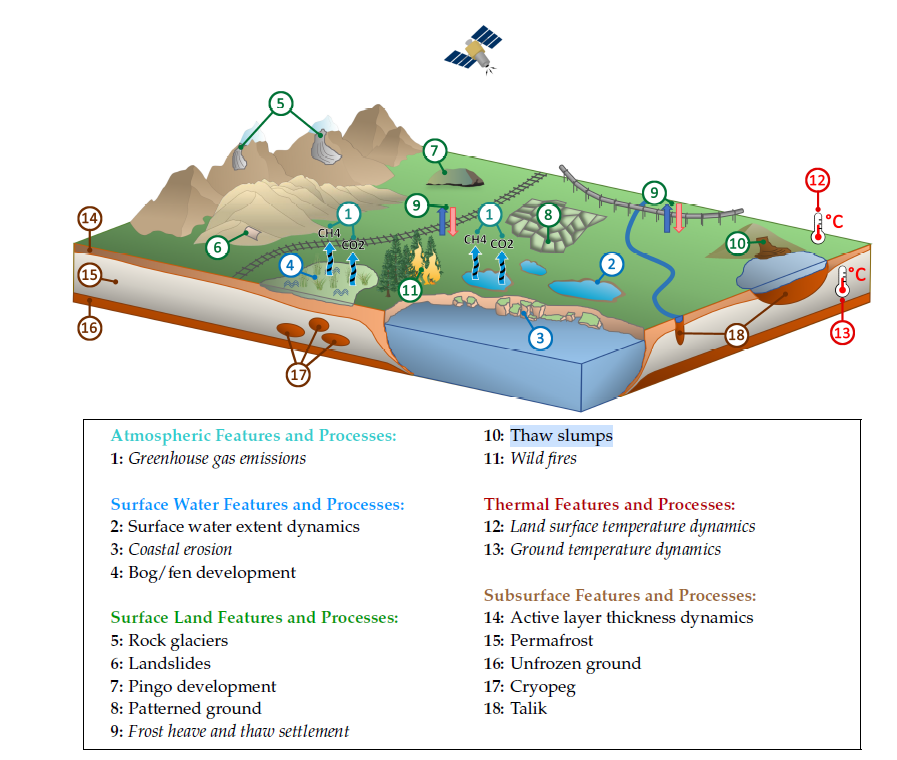
\includegraphics[width=1 \textwidth]{fig 1 thermokrast landform.png}
        \caption{Landscape features and processes info-graphic (\cite{rs13061217})}
        \label{fig_thermokrast}
    \end{figure}



\subsection{Retrogressive Thaw Slumps}  \label{rts_intro}

\paragraph{}
\gls{RTS}s can usually be described as horseshoe-shaped landslides caused by the thawing of ice-rich permafrost, which causes erosion mostly at its steep head scarp. \gls{RTS} usually occur on sloped terrain so that the thawed material can flow downslope, usually into nearby water features such as lakes and rivers. (\cite{articleperma})
 
This means that \gls{RTS}s have particular parts that can ease their visual identification through the mentioned head scarp, the headwall that forms after the slump, the slump floor itself (\cite{LANTUIT200884}) which is also described as slump scar zone. These have been labeled in Figure \ref{fig_RTS} for the reader's benefit. 

    \begin{figure}[hbt!]
        \centering
        \includegraphics[width=1 \textwidth]{RTS.png}
        \caption{Example of an \gls{RTS} with added legend. (b) and (c) are the
ground photo and remote sensing image of an \gls{RTS} whose central location is 92.912° E, 34.848° N. (\cite{HUANG2020111534})}
        \label{fig_RTS}
    \end{figure}


As some sections of the slump scar stabilise they become vegetated (\cite{KOKELJ201556}) and thus harder to identify using only visual Red (R), Green(G) and Blue (B) channels, this is where remote sensing's other "sensor" bands can identify other features not seen with the "naked eye" (\cite{HUANG2020111534})
\section{Artificial Intelligence Applications in Remote Sensing}  \label{ai_rs}
\paragraph{}
The advancements in Artificial Intelligence have made it possible to identify and classify particular features in images and like in this case, even remote sensing imagery, this section will introduce the techniques used in this field.

Given the lack of research found on the specific task of identifying \gls{RTS}s using remote sensing imagery, a more expansive approach on looking at \gls{DL} and \gls{ML} techniques using remote sensing imagery was taken.

\subsection{Conventional \gls{ML} applications in Remote Sensing}  \label{ml_rs}
\paragraph{}
Before the rise in popularity of \gls{DL} applications in Remote Sensing imagery, more shallow structures that process features extracted from the sattelite images,such as \gls{RF}, were used. This type of \gls{ML} require features to be extracted by experts and flattened to enable the algorithm to use them, this can be time consuming and can be overcome by the use of \gls{DL}, which does the feature map extraction as part of the algorith as will be seen in section \ref{cnn_layers}.

In a study (\cite{isprs-archives-XLII-3-79-2018}) on extracting built-up areas from Sentinel-2 remote sensing imagery, \gls{DL} techniques were compared against the most widely used conventional \gls{ML} methods in remote sensing classification to show the benefits of usng \gls{DL} algorithms, both Gaussian \gls{SVM} and \gls{BPNN} were evaluated.

\paragraph{\gls{SVM}}
\paragraph{}
According to a 2010 review (\cite{MOUNTRAKIS2011247}) of over 100 studies on the use of \gls{SVM} in remote sensing, this model's popularity in the field came from its ability to generalise well even when there is limited training data, which is quite common in remote sensing problems. Their major limitation comes in the form of parameter assignment issues, which affect the quality of the results.

\paragraph{\gls{RF}}
\paragraph{}
\gls{RF} has always been a popular method, as it is an ensemble classifier that makes use of multiple decision trees combined with random subsampling of the training data and variables. 

According to a review on the use of \gls{RF} in remote sensing, (\cite{BELGIU201624}) \gls{RF} became a popular classifier in remote sensing due to the high accuracy of its classifications. It also seems to successfully handle the high dimensionality and multicollinearity of remote sensing data, as well as, being fast and not prone to overfitting. Its main limitation is its sensitivity to the sampling design.

\paragraph{\gls{BPNN}}
\paragraph{}
The traditional \gls{BPNN} is a popular \gls{ML} algorithm, according to a review (\cite{YUAN2020111716}) in environmental remote sensing it has been used extensively for research in this field. Yuan et al. reports improvement in accuracy against traditional regression methods across a number of papers by using \gls{BPNN}, but highlights a couple of limitations: the slow convergence of the algorithm and how much it is affected by weight initialisation being susceptible to getting stuck in local minimums. 

This traditional Neural Network forms the back-bone of many \gls{DL} models, so it is important to understand its inner works.

A \gls{BPNN} consists of one or more hidden layers between an input and an output layer, each layer having many neurons/nodes that are fully connected to the next layer as it can be seen from Figure \ref{fig_bpnn}.  It is trained via forward and backward propagation, that is: starting with forward propagation, the input is propagated through the hidden layers in the network until it reaches the output layer where the error between the predicted and actual values is calculated. 

Straight after the error is calculated, it is propagated backward to update the neuron weights of each layer to minimise the error.

    \begin{figure}[hbt!]
        \centering
        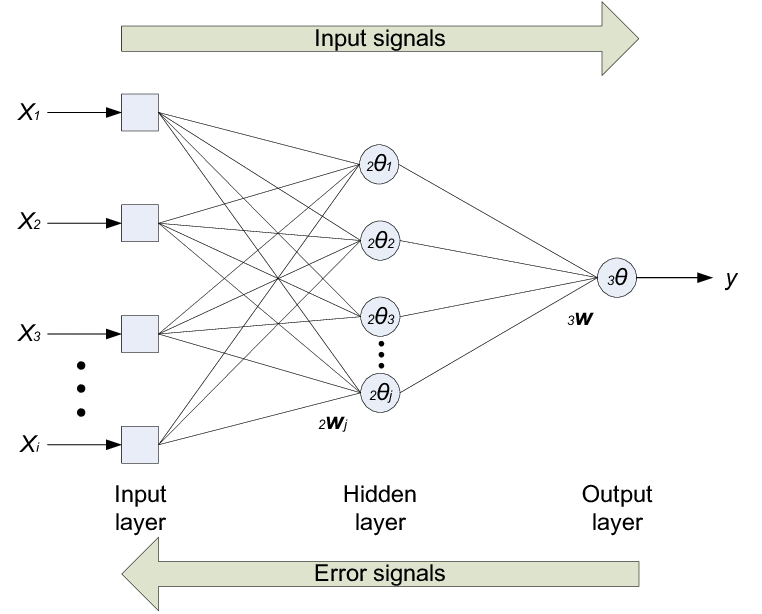
\includegraphics[width=0.5\textwidth]{Three-layer-back-propagation-neural-network.png}
        \caption{Three-layer back-propagation neural network (\cite{NNpic})}
        \label{fig_bpnn}
    \end{figure}

\subsection{\gls{DL} applications in Remote Sensing Imagery} \label{dl_rs}
\paragraph{}
Looking at the field of \gls{DL} with Remote Sensing, most studies have been focused on the field of \gls{LULC} classification, as suggested by a \gls{DL} in Remote sensing application review (\cite{MA2019166}) in Figure \ref{fig_dl_studies}. Object detection, Scene Classification and Segmentation (\gls{a.k.a.} pixel-wise classification) are also techniques to classify images or areas of these images.

    \begin{figure}[hbt!]
        \centering
        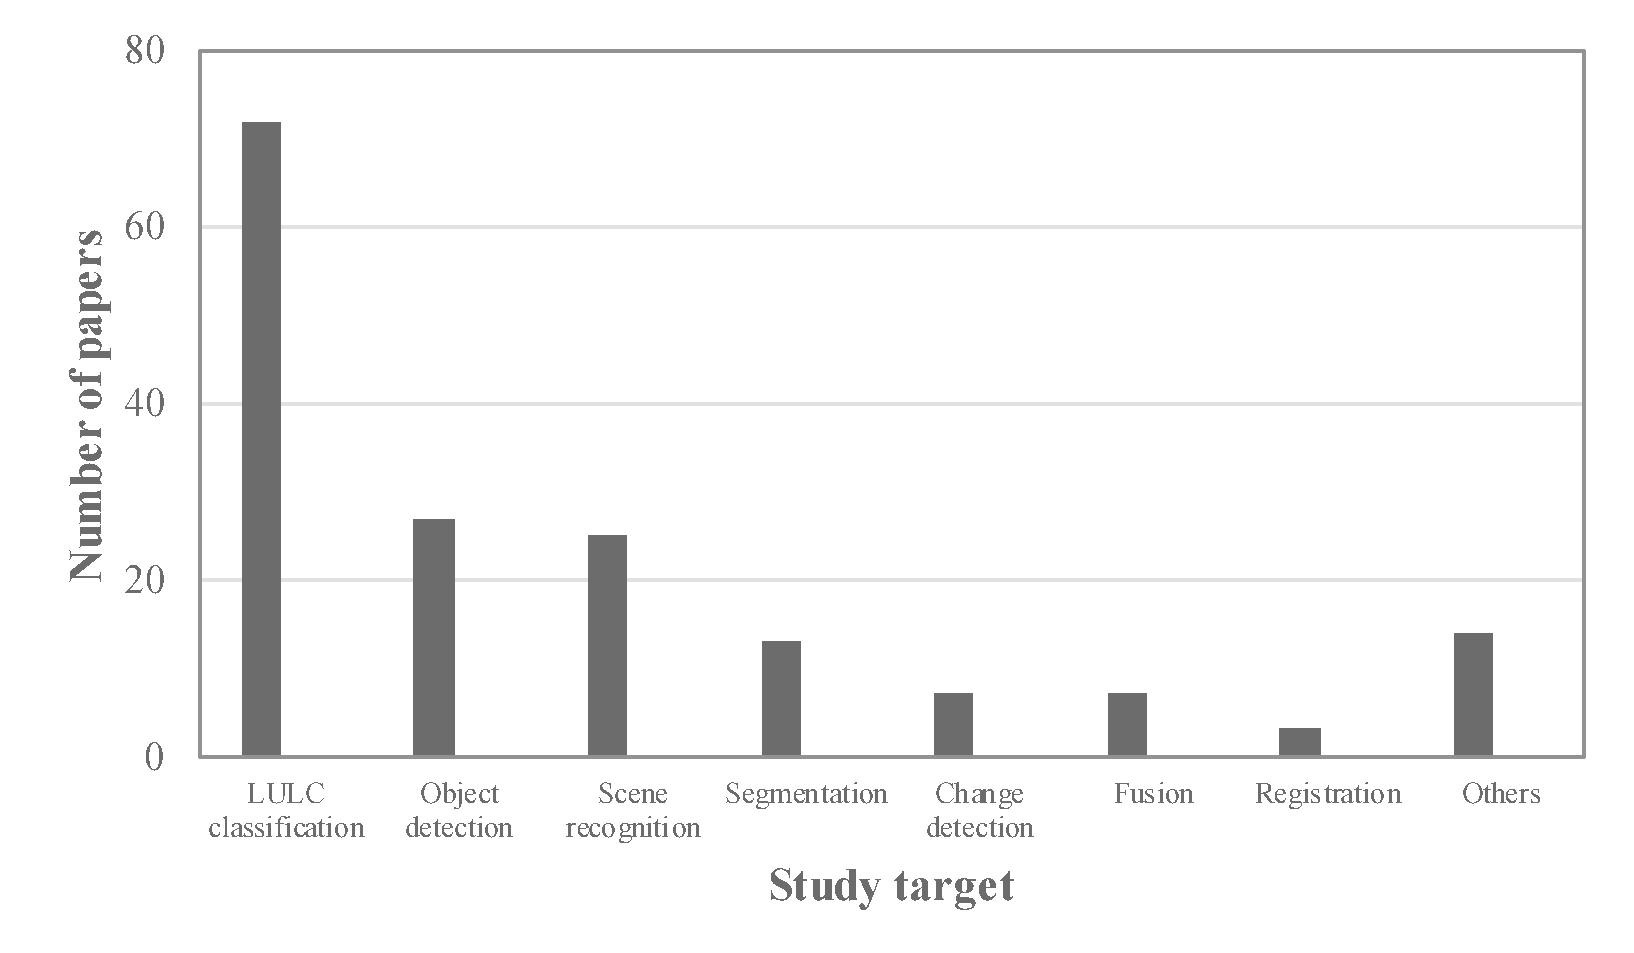
\includegraphics[width=0.75\textwidth]{study_target_ma.jpg}
        \caption{Study target of \gls{DL} in Remote Sensing studies (\cite{MA2019166})}
        \label{fig_dl_studies}
    \end{figure}

In traditional natural images, image classification is the task of assigning a label to a whole input image, either by outputting a class or a probability of tasks that describe said image. However, this is not the case in remote sensing, where the concept is broader, referring to either pixel-wise or "scene" classification, as shown in Figure \ref{fig_img_class_frame}.

\paragraph{Pixel-wise classification} The classification of each pixel, similar to the concept of image segmentation, as it is known when performed in natural images. Each pixel in a remote sensing image could represent, as an example, a 10 by 10 meter area, which would usually be associated with a natural image area. 

So by classifying each pixel in a remote sensing image, we are classifying a 10x10 meter area, each class for example represented by the different colours at the top right of Figure \ref{fig_img_class_frame}. 

\paragraph{Scene classification} The automatic assignment of a semantic label to a scene, represented by the different coloured "containers" at the bottom right of Figure \ref{fig_img_class_frame}. A scene being a local image patch, usually manually extracted from large-scale satellite images that contain classes (e.g. forest areas, residential area)(\cite{https://doi.org/10.1002/widm.1264}).

    \begin{figure}[hbt!]
        \centering
        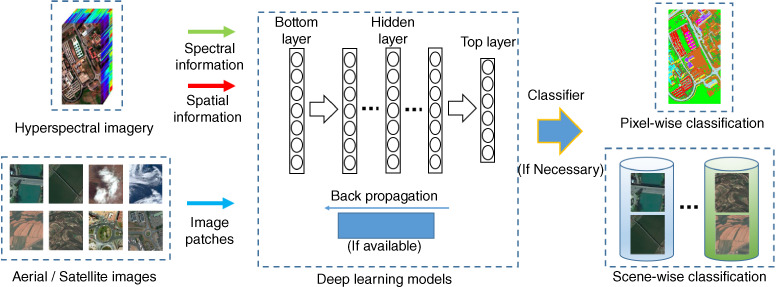
\includegraphics[width=0.8\textwidth]{widm1264-toc-0001-m.jpg}
        \caption{General Framework of Remote Sensing Image Classification Based on \gls{DL} (\cite{https://doi.org/10.1002/widm.1264})}
        \label{fig_img_class_frame}
    \end{figure}


\paragraph{Object detection} In remote sensing images, it is used to find out if a satellite image has one or more objects belonging to a given class and find the position of each object predicted in the image.(\cite{CHENG201611})

\subsection{\gls{DL} Models in Remote Sensing} \label{dl_models_rs}
\paragraph{}
The same review (\cite{MA2019166}) also suggests that the most used \gls{DL} model in Remote Sensing imagery is \gls{CNN} as indicated in Figure \ref{fig_dl_rs}.
    \begin{figure}[hbt!]
        \centering
        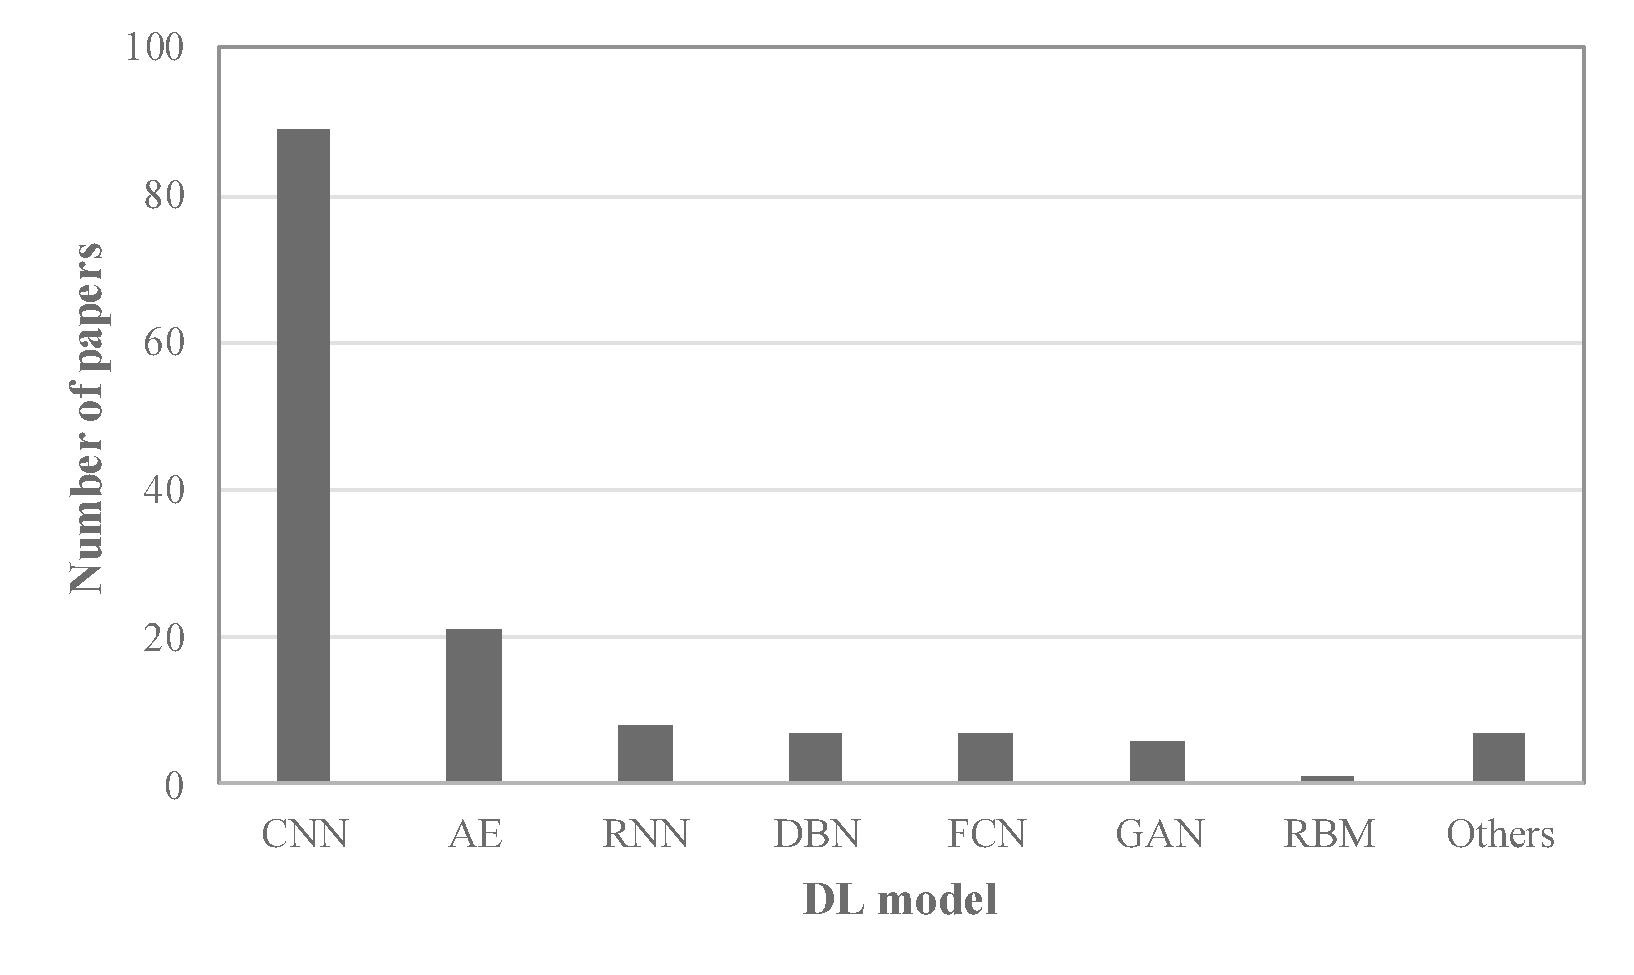
\includegraphics[width=0.75\textwidth]{DL_MA.jpg}
        \caption{\gls{DL} models used in Remote Sensing studies (\cite{MA2019166})}
        \label{fig_dl_rs}
    \end{figure}
    
The models in Figure \ref{fig_dl_rs} can be classified into two types of \gls{DL} models:
\gls{CNN}, \gls{RNN}, and \gls{FCN} are supervised models, whereas \gls{AE}, \gls{DBN}, \gls{GAN} models are unsupervised models. 

Supervised models require labeled data to learn from the ground truth, whereas unsupervised ones don't.  For example, Alvarez et al. (\cite{alvarez2020s2cgan}) use \gls{GAN} to solve the binary change detection problems in remote sensing by exploiting the discriminator likelihood to generate the distribution of unchanged samples.

As labeled data has been collected for this project, its focus will be on a supervised \gls{DL} Model. \gls{CNN} has been chosen as its the most popular supervised techniques, section \ref{cnn_subsect} will expand on this.

%Expand on these?     
% \paragraph{Auto Encoders}
% \paragraph{Deep Belief Networks} 
 % \paragraph{RNN}  
% \paragraph{GAN}


\section{\gls{CNN}} \label{cnn_subsect}
\paragraph{}
\gls{CNN}s are a type of \gls{ANN} that have been praised for their contribution to the field of computer vision. \gls{CNN}s have been very successful and efficient in image classification, object detection, and many other computer vision applications (\cite{GoodBengCour16}).

In general, a \gls{CNN} takes an input image, extracts low-level features, and hierarchically builds on this to extract more abstract features, so that it is able to extract features that are common for all outputs. This concept has its origin in the biology of the visual cortex, which has small regions of cells that "light up" to specific characteristics of the visual field until the entire visual field is processed and categorised.

\subsection{Main Layers of a \gls{CNN}} \label{cnn_layers}
\paragraph{}
Like any other Neural Network, a \gls{CNN} is composed of an input layer, an output layer, and several hidden layers connecting them, as shown in Figure \ref{fig_cnn_layers}.

The input layer usually consists of a representation of the input image to be analysed, and the output layer of the probabilities for each class.
The hidden layers usually consist of convolutional, non-linearity, pooling, and fully connected layers, which are the building blocks for most \gls{CNN}s and therefore will be described in detail below.

    \begin{figure}[hbt!]
        \centering
        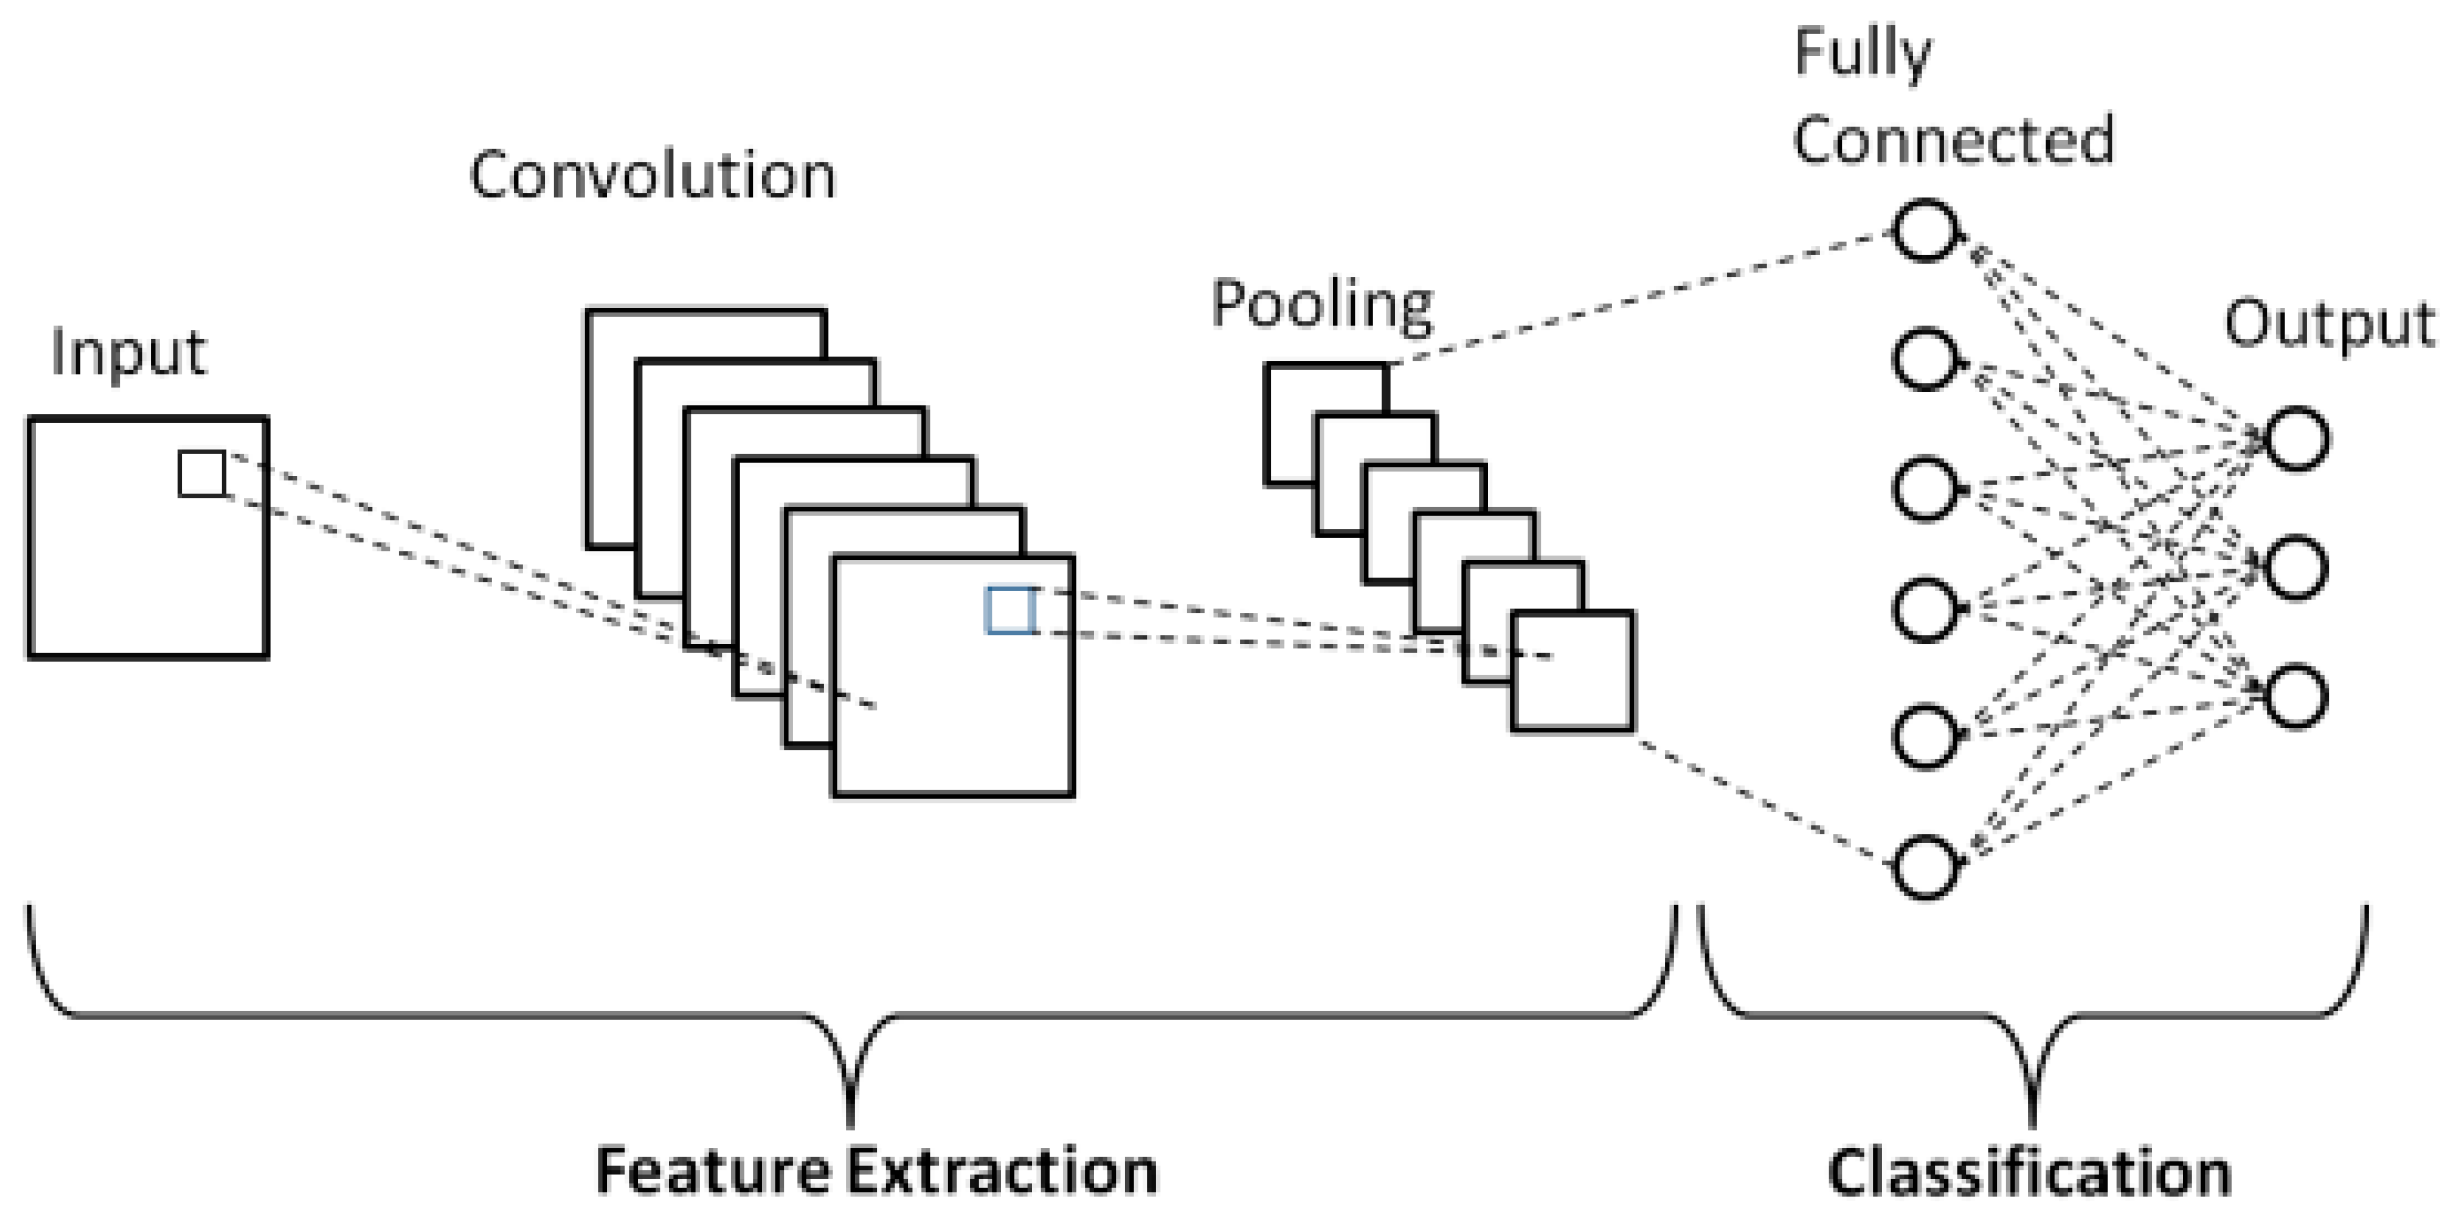
\includegraphics[width=0.75\textwidth]{cnnclassification.png}
        \caption{The main layers of a \gls{CNN} (\cite{10.6109/JICCE.2018.16.3.173})}
        \label{fig_cnn_layers}
    \end{figure}

\subsubsection{Input Layer}
\paragraph{}
Each image is represented as a 3D matrix with dimensions of  width (W), height (H), and depth (D), respectively. In the field of natural images the third dimension, depth, may take the value of 3 for \gls{RGB} channels of images, or one for grey colour images. However, in the field of remote sensing imagery this dimension can have N channels each associated with readings from a different sensor. For example Sentinel-2 images have 13 channels, this will be explored in detail in section \ref{sentinel2_section}. 

\subsubsection{Convolutional Layer}
\paragraph{}
The objective of the Convolution Operation, after which the layer has been named, is to extract features from an image. It is the key differentiator from a Dense layer, as it enables the ability to capture dependencies between pixels through the application of filters. It learns local patterns rather than global patterns.
In abstract mathematical terms, it takes the matrix of the image and the matrix of a filter/kernel and merges the information in both. By making the filter smaller than the input dimension, sparse interaction can be achieved, reducing the memory requirements and improving the model's  efficiency.

It also means that neurons are constrained to using the same set of weights for getting the output, \gls{a.k.a.} shared parameters. This parameter sharing gives the Convolution Operator the property of translation equivariance, meaning that if we translate the input the output will also be translated, giving \gls{CNN}s the ability to learn features regardless of their position.

A Convolutional layer is a layer that applies different convolution operations to the data, making it the most essential building block of a \gls{CNN}, and its most computationally expensive one as well. To fully understand this process, it will be broken down below.

The filter/kernel, introduced above has dimensions ($K$) smaller than the input image for height and width but the same third dimension, the number of channels ($n$). The filter moves along the width and height of the input image, with a certain stride ($s$) value, performing matrix multiplication between the filter and the same dimensional portion of the image over which the filter is passing (depicted by the shaded area in Figure \ref{fig_cnn_filter}) until it traverses the entire image.

    \begin{figure}[hbt!]
        \centering
        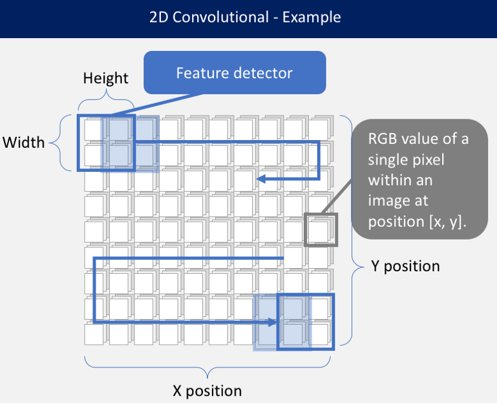
\includegraphics[width=0.5\textwidth]{2DCNN.jpg}
        \caption{The movement of the filter in a 2D \gls{CNN} layer (\cite{2dcnnpic})}
        \label{fig_cnn_filter}
    \end{figure}
     
In the case of images with $n$-channels, the matrix multiplication is performed between the kernel and input channel stacks as depicted in Figure \ref{fig_cnn_conv}, all the results are then summed with the bias to give a one-depth channel convoluted feature map with depth equal to the number of filters ($m$).

    \begin{figure}[hbt!]
        \centering
        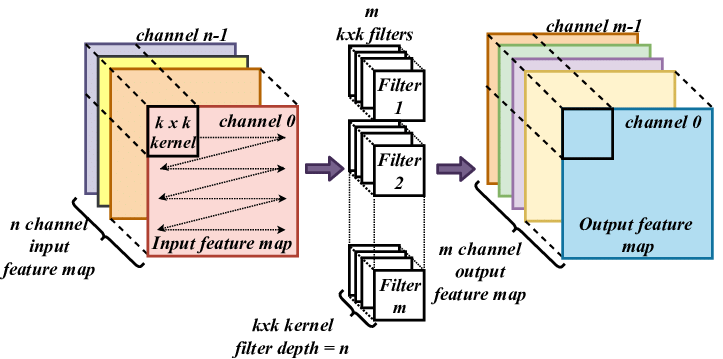
\includegraphics[width=0.75\textwidth]{Convolution-operation-in-a-CNN.png}
        \caption{The Convolution Operation in an n-channel input \gls{CNN} (\cite{9053228})}
        \label{fig_cnn_conv}
    \end{figure}
      
The size of this feature map will be affected by several parameters, some of which have been mentioned above already:

\begin{itemize}
    \item \textbf{Filter dimensions ($K$)} The dimensions of the filters used in the layer. For example, $k$ x $k$ x $n$ in Figure \ref{fig_cnn_conv}.
    \item \textbf{Stride ($s$)} The number of pixels the filter shifts over the input matrix. When the stride is 1, the filters are moved 1 pixel at a time. The larger the stride, the smaller the feature map.
    \item \textbf{Number of filters ($m$)} The number of filters used in the convolutional layer. It is said that the higher the number of features the more image features get extracted and the better the \gls{CNN} gets at recognising patterns in unseen images.
    \item \textbf{Zero Padding ($p$)} Sometimes the filter dimensions don't fit the image input dimensions perfectly. A strategy commonly used to maintain the input matrix dimensions and avoid the loss of information is to pad said matrix with 0s around the borders.
\end{itemize}
  
The output convolution dimensions, assuming a symmetric \gls{CNN} architecture and image to be square that is height equals width, so both dimensions have the same values, can be calculated as follows (\cite{dumoulin2018guide}):

\begin{equation}
    \label{conv_dim_eq}
    dim_{out} = \frac{dim_{in} + 2p - K}{s} + 1
\end{equation}

If either the architecture or the input size is asymmetric, \ref{conv_dim_eq} can be used to calculate the feature map dimensions separately for height and depth.

When it comes to depth as shown in Figure \ref{fig_cnn_conv}, the output depth dimension is always equal to the number of filters $m$:

\begin{equation}
    \label{conv_depth_eq}
    D_{out} = m
\end{equation}

A \gls{CNN} will usually have several convolutional layers to learn spatially hierarchical patterns. The first convolutional layer will learn local simple patterns such as lines and edges, then a second convolutional layer will learn features made up of the features learned in the first layer to learn more complex patterns. 

As we go deeper into the network, the filters also begin to be more responsive to a larger region of the pixel space, enabling it to learn larger patterns. The process will repeat itself for subsequent layers, the number of layers will depend on the complexity of the input image's features.

\subsubsection{Non-Linearity Layer}
\paragraph{}
Non-linearity is a key feature of \gls{NN} that enables the modelling of outputs that can't be produced from linear combinations of the inputs.
A non-linearity layer is nothing more than an activation function that takes the feature map generated by the convolutional layer and creates an activation map as the output. 

The different activation functions are described in section \ref{cnn_activation} in detail. Most of the recent \gls{CNN} meta-architectures use \gls{ReLU} (or its derivatives, such as leaky \gls{ReLU}s) due to their efficiency and robustness to noise (\cite{he2015delving}).

\subsubsection{Pooling Layer}
\paragraph{}
The Pooling Layer, \gls{a.k.a.} subsampling or downsampling layer, usually follows a Convolutional Layer or a Non-Linearity Layer if these are separate. 
Its main function is to reduce the dimensionality and subsequently the number of parameters in the network, whilst retaining the most important information of the activation map. This can reduce the training time/ computational power required and increase training efficiency through extracting the dominant translation-invariant features.


Just like the convolutional layer above, a window slides through each feature map applying the pooling operation, so spatial neighbourhood dimensions/ pooling kernel size ($K_p$) and stride ($s$) are important parameters that need to be defined beforehand. For example, in an overlapping pooling layer $K_p > s$, one can calculate the feature map output dimensions following a pooling layer as follows (\cite{dumoulin2018guide}) using equations \ref{pool_dim_eq} and \ref{pool_depth_eq}:

\begin{equation}
    \label{pool_dim_eq}
    dim_{out} = \frac{dim_{in} - K_p}{s} + 1
\end{equation}

When it comes to depth, the output depth dimension is always equal to the input dimension depth:

\begin{equation}
    \label{pool_depth_eq}
    depth_{out} = depth_{in}
\end{equation}

To achieve this, several spatial pooling types can be applied interchangeably, the most common ones are described below. Figure \ref{fig_pooling} depicts an example of a non-overlapping pooling layer, where $K_p = s$:

\begin{itemize}
    \item \textbf{Max Pooling} It returns the maximum value from the window of the image covered by the pooling kernel. It discards noisy activations, thus performing de-noising as well as dimensionality reduction. This could help avoid overfitting. In practice, this type of pooling shows the best performance (\cite{GoodBengCour16}).
    \item \textbf{Average Pooling} It returns the average of all the values from the window of the image covered by the pooling kernel, only performing dimensionality reduction.
\end{itemize}

    \begin{figure}[hbt!]
        \centering
        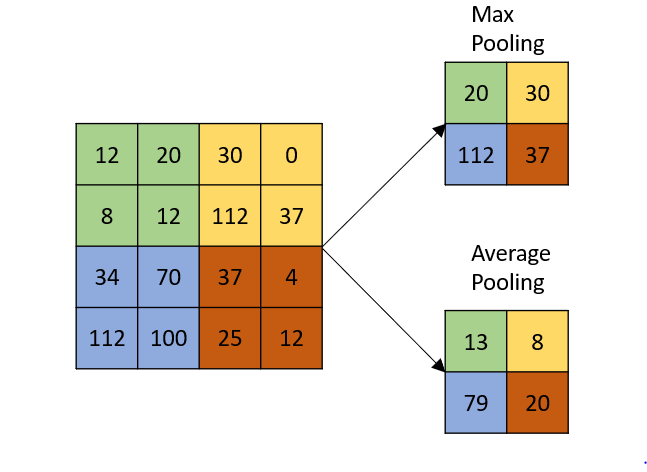
\includegraphics[width=0.5\textwidth]{pooling_diagram.png}
        \caption{Different types of pooling with 2x2 kernel and stride 2}
        \label{fig_pooling}
    \end{figure}
    

\subsubsection{Fully Connected Layer}
\paragraph{}
Finally, once the outputs of all the layers above successfully represent the high-level features of the input image, this output is flattened into a 1D matrix that can be fed to the Fully Connected Layers. The first few layers of this type learn non-linear combinations of these features to identify which of these features most strongly correlate with the output classes.

In a scene classification problem, to identify the most likely output class, the last of these fully connected layers usually has a softmax (multi-class problem)  or sigmoid (binary class problem) activation function to output a $1$x$N$ matrix of probabilities, with each element in this matrix corresponding to the probability of an object belonging to a specific class and all of these probabilities summing to one.

In a pixel-wise classification problem, the final layer could be used to perform a pixel-wise prediction and will output a $W$x$H$ matrix of probabilities, with each element in this matrix corresponding to the probability of an object belonging to a specific class. More detail on how the necessary $W$x$H$ dimensions are upsampled is given in the following layer.

\subsubsection{Fractionally-strided/ Transposed Convolutional Layer}
\paragraph{}
For example, in an architecture that allows for end-to-end pixel-wise classification, such as \gls{FCN}), a fractionally-strided layer (\cite{long2015fully}) is needed to link the network's outputs back to the pixels  using learnable parameters. It is used to upsample the feature map within the network back to the image size dimensions as a segmentation map to enable end-to-end learning by backpropagating the pixel-wise loss. It is often misleadingly  referred to as deconvolutional layer, due mainly to its use in a study (\cite{zeiler2013visualizing}) that visualises convolutional networks. 

In a pixel-wise classification problem, this could also be used as the last layer, like in Deconvnet (\cite{7410535}) instead of feature maps this Transposed Convolutional Layer generates pixel-wise class probabilities corresponding to the size of the input images, the said $W$x$H$ matrix described above.

\subsection{Activation Functions} \label{cnn_activation}
\paragraph{}
There are several activation functions used for different purposes, those commonly used in hidden layers are the Tahn, Sigmoid, and \gls{ReLU} activation functions.
In a \gls{CNN}, it is usual to have an activation function following every convolution layer to introduce non-linearity, the recommendation in modern \gls{NN} is the use of \gls{ReLU} activation functions(\cite{GoodBengCour16}).

We will start by introducing some activation functions commonly used in the output layer - softmax and sigmoid.

\subsubsection{Softmax}
\paragraph{}
Anytime we want to represent a probability distribution over a discrete variable with K possible values we use the softmax function shown in Equation \ref{sofmax_eq}. It can be thought of as a generalisation of the Sigmoid function shown in Equation \ref{sigmoid_eq}, which is used to represent it over a binary variable instead (\cite{GoodBengCour16}).

\begin{equation}
    \label{sofmax_eq}
    \sigma(z_i) = \frac{e^{z_{i}}}{\sum_{j=1}^K e^{z_{j}}} \ \ \ for\ i=1,2,\dots,K
\end{equation}

In \gls{NN}, the softmax activation function is commonly used for multi-class classification, being an output layer that predicts the multinomial probability distribution described above.

As it can be seen in Figure \ref{fig_softmax}, the softmax activation will output one value for each node in the output layer, this outputted vector of probabilities that sum to $1$, is interpreted as the probability of membership for each class.

\begin{figure}[hbt!]
    \centering
    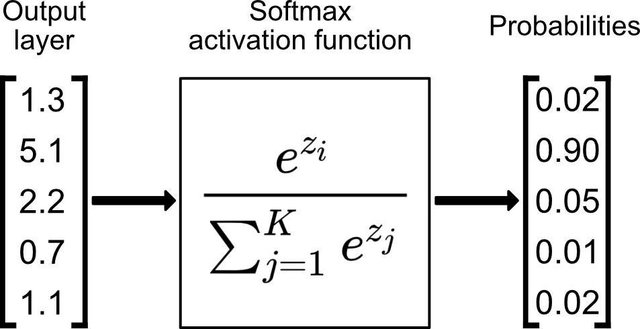
\includegraphics[width=0.4\linewidth]{softmaximg.jpg}
    \caption{Softmax activation function (\cite{softmaxpic})}
    \label{fig_softmax}
\end{figure}

\subsubsection{Sigmoid}
\paragraph{}
Although the Sigmoid activation function was popular in the 90s as a non-linear layer to normalise the output of each neuron in hidden layers, it lost popularity (\cite{GoodBengCour16}) to both the activation functions that follow.

These days, since it outputs values between 0 and 1, the sigmoid activation function is usually used in the output layer for single label/ multi-label binary classification problems. 

\begin{equation}
    \label{sigmoid_eq}
    % sigmoid(x) = \frac{1}{1 + e^{-\alpha x}} 
    \sigma(z) = \frac{1} {1 + e^{-z}}
\end{equation}


\subsubsection{Tanh}
\paragraph{}
The hyperbolic tangent activation function \gls{a.k.a.} Tanh function was used as the default activation function for hidden layers in the late 90s to 2010s after it showed signs of typically performing better than the logistic sigmoid activation function (\cite{GoodBengCour16}).
Both of these activation functions are depicted in Figure \ref{fig_tahn_sigmoid}.

As shown in Equation \ref{tanh_eq}, it takes as input any real value and outputs values between -1 and 1.

\begin{equation}
    \label{tanh_eq}
    Tanh(x) = \frac{1 - e^{-\alpha x}}{1 + e^{-\alpha x}} 
\end{equation}

Despite their ability to learn complex mapping functions, both the Sigmoid and Tahn activation functions have a known limitation, they saturate for extreme values of z, only being strongly sensitive to their input when z is near 0, which can be seen from Figure \ref{fig_tahn_sigmoid}. 

This problem is known as vanishing gradients, it makes it very difficult to know how the parameters should change to improve the cost function (\cite{GoodBengCour16}) and consequently for Deep Neural Networks to learn effectively.

\begin{figure}[hbt!]
    \centering
    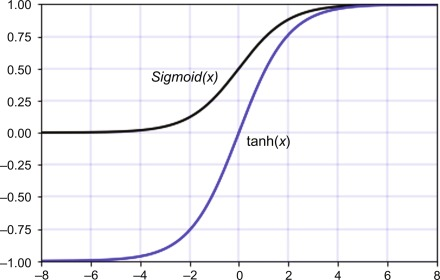
\includegraphics[width=0.5\linewidth]{tahn sigmoid funciton.jpg}
    \caption{Tahn and Sigmoid activation functions (\cite{tahnfunc})}
    \label{fig_tahn_sigmoid}

\end{figure}

\subsubsection{\gls{ReLU}}
\paragraph{}
\gls{ReLU}s were introduced to address the problem of vanishing gradients and quickly replaced the Sigmoid and Tahn activation functions by providing  performance improvements, Deep \gls{CNN}s with \gls{ReLU}s trained several times faster than the same ones with Tahn units(\cite{GoodBengCour16}).

The rectified linear activation function simply returns the input value provided if this value is greater than 0, or the value 0 if the input is 0 or less.

\begin{equation}
    \label{eq_relu}
    Relu(z) = max(0, z)
\end{equation}

In this sense, it can be said that because \gls{ReLU}s are nearly linear, they preserve properties that make linear models easy to optimise and generalise well (\cite{GoodBengCour16}).

\gls{ReLU}s do not come without limitations, large updates to the weights could mean that the input to the activation function is always negative, therefore the activation value will always be $0$, this is known as the dying \gls{ReLU} problem.
This means the gradient is $0$, so the unit will never activate, the weights will not be adjusted, so like the vanishing gradient problem the learning will be slow with constant 0 gradients (\cite{Maas13rectifiernonlinearities}).

This can be corrected by several variations of the \gls{ReLU}, for example Leaky and Parametric \gls{ReLU}s  that change the slope to the left of $x < 0$. Either by a fixed parameter in Leaky \gls{ReLU} as shown in Figure \ref{fig_relu} or by a parameter that is learned by backpropagation using weights and biases in Parametric \gls{ReLU}. 

There are more complex examples like \gls{ELU}s  and Threshold \gls{ReLU} functions that are known to improve accuracy compared to \gls{ReLU}s.

\begin{figure}[hbt!]
        \centering
        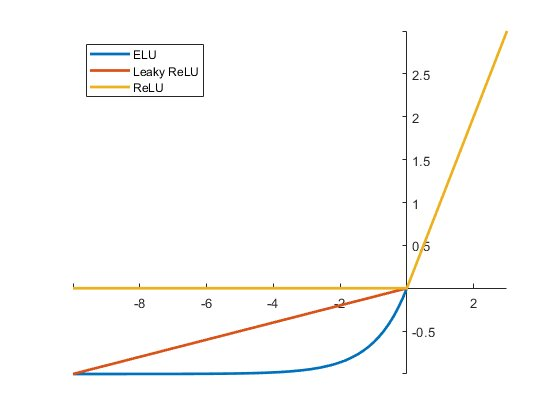
\includegraphics[width=0.65\linewidth]{RELU variations.jpg}
        \caption{Rectified Linear activation functions (\cite{leakyreluimg})}
        \label{fig_relu}
\end{figure}

\subsection{Classical \gls{CNN} Architectures and their evolution} \label{classic_cnn}
\paragraph{}
An architecture is the arrangement of the layers introduced thus far into set patterns. The first \gls{CNN} architecture was introduced by Lecun in the early 90s, followed by some other influential architectures that have built on each other and evolved since. This section describes these and their contributions.

\subsubsection{LeNet}
\paragraph{}
In 1989, LeCun et al. proposed the first multilayered \gls{CNN} successfully trained via backpropagation. After a decade of improvement iterations, LeNet-5 (\cite{726791}) was the famous architecture depicted below that started the use of \gls{CNN}s for Optical Character Recognition (OCR) tasks, but it didn't perform well in other computer vision problems.

    \begin{figure}[hbt!]
        \centering
        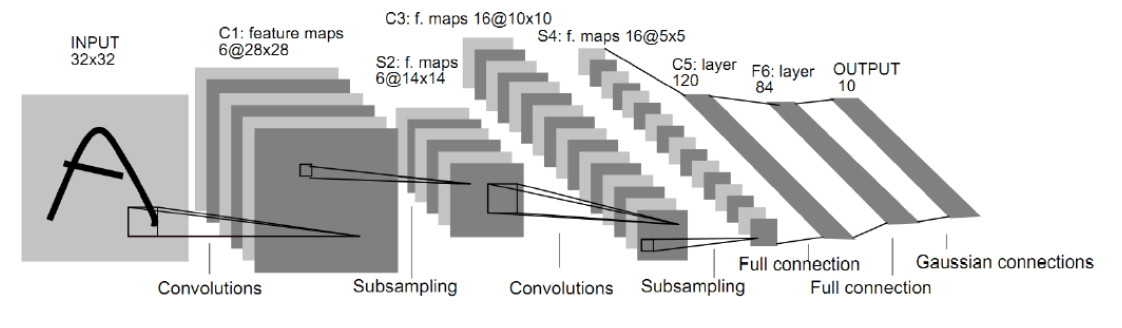
\includegraphics[width=0.75\textwidth]{lenet_arch.png}
        \caption{Architecture of LeNet-5 (\cite{726791})}
        \label{fig_lenet}
    \end{figure}
    
\subsubsection{AlexNet}
\paragraph{}
In 2012, Krizhevsky et al.(\cite{10.5555/2999134.2999257}) took LeNet's work as inspiration to create a much deeper \gls{CNN} and implemented a few novel contributions which are still essential to the success of \gls{CNN}s to this day:
\begin{itemize}
    \item \textbf{\gls{ReLU}s} The benefits of these have been highlighted in section \ref{cnn_activation}, contributing to faster training times than the Sigmoid activation function used in LeNet's implementation.
    \item \textbf{Dropout} The use of Dropout layers as a regularisation method helped avoid the problem of overfitting
    \item \textbf{Data Augmentation} Using artificial data augmentation techniques to increase the size and variety of the training dataset by translating and reflecting existing images improved the performance of the model
     \item \textbf{Training on a \gls{GPU}} Using a couple of \gls{GPU} to train AlexNet allowed for faster training on great amounts of bigger images which set a milestone for the success of \gls{CNN}s, the delineation of responsibilities between the 2 \gls{GPU}s is shown in Figure \ref{fig_alexnet}.
\end{itemize}

    \begin{figure}[hbt!]
        \centering
        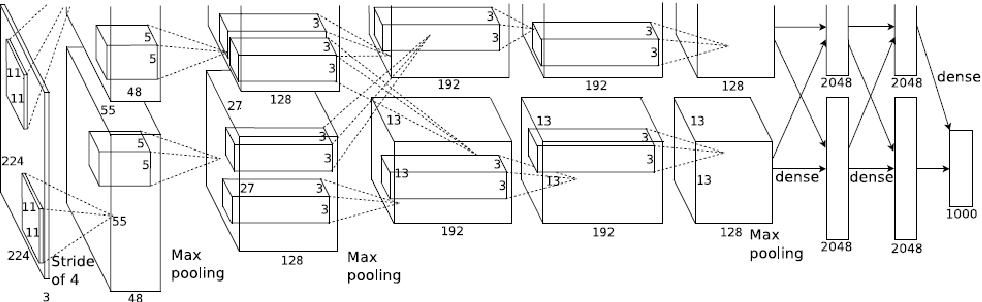
\includegraphics[width=0.75\textwidth]{alexnet_arch.png}
        \caption{Architecture of AlexNet (\cite{10.5555/2999134.2999257})}
        \label{fig_alexnet}
    \end{figure}


\subsubsection{VGG}
\paragraph{}
VGGNet (\cite{simonyan2014deep}) won the ImageNet Challenge 2014. This network is built on the simple principles of the two conventional \gls{CNN}s introduced above, creating a deeper network (19 weight layers) with the idea of using blocks of an increasing number of filters. These repeated structures of a sequence of convolutional layers followed by a max-pooling layer for downsampling, create deeper networks with more non-linearities captured. Several other factors contributed to its success:

\begin{itemize}
    \item \textbf{Filters with smaller dimensions} By using filters with a smaller receptive field of 3x3 and maintaining the number of filters in each of the convolutional layers in the same block, in a sequence of layers, more non-linearities can be captured using fewer parameters.
 
    \item \textbf{Increasing number of filters} By roughly doubling the number of filters in each block, more complex features can be captured
    \item \textbf{Scale jittering} Uses scale jittering as one of the data augmentation techniques.

\end{itemize}

\subsubsection{Other Evolutions}
\paragraph{}
Several meaningful contributions were made by other architectures, such as:

\begin{itemize}

    \item \textbf{\gls{NiN}}  A \gls{NiN} block(\cite{lin2014network}) applies a fully-connected layer to each pixel, they consist of a convolutional layer and multiple 1x1 convolutional layers, this design has influenced many other \gls{CNN} designs.
 
    \item \textbf{GoogleNet } Also working with blocks, each of its "Inception" (\cite{7298594}) blocks has 4 paths, extracting information in parallel through convolutional layers of different filter dimensions and max-pooling layers. It also makes use of the 1x1 convolution introduced in \gls{NiN} to reduce channel dimensionality per pixel. This makes it a very efficient network architecture with a low computational cost.
    
    \item \textbf{Batch normalisation )} Introduced in 2015, this method (\cite{ioffe2015batch}) makes normalisation part of the model architecture by performing it for each training mini-batch. It performs reparametrisation of the model, reducing the need to coordinate updates across many layers (\cite{GoodBengCour16}). It not only allows the use of much higher learning rates and more relaxed initialisation, but it also acts as a regularisation technique, as will be seen in section \ref{regulariser}.
    
    \item \textbf{ResNet} This architecture (\cite{he2015deep}) challenges the convention of optimising the original unreferenced functions by optimising the residual mappings instead. This way the authors manage to create residual networks with a depth of 152 layers, which is 8 times deeper than the VGG net whilst keeping a lower complexity, making them more accurate and easier to optimise. 
    \item \textbf{DenseNet} This architecture (\cite{8099726}) builds on the concept of the ResNet but instead of adding inputs and outputs together in its cross-layer connections, it concatenates them instead. It also uses transition layers (1x1 convolution) to keep the dimensions under control.

\end{itemize}

\section{The various architectures used in Remote Sensing applications} \label{seg_nets}
In the field of Remote Sensing applications, the goal is usually pixel-wise classification, which can be thought of as natural image segmentation. For this, the main state-of-the-art \gls{CNN}-based segmentation models used in remote sensing have been introduced.

\subsection{\gls{FCN}} 
\paragraph{}
Long et al. (\cite{long2015fully}) proposed \gls{FCN} to address the task of semantic segmentation. Having taken as base models some Classical \gls{CNN} architectures introduced in Section \ref{classic_cnn}, these were transformed from classifiers to \gls{FCN} by swapping the fully connected layers with convolutional layers and dropping the final classifier layer. 

Maggiori et al. (\cite{7730322}) celebrates the improvements of using \gls{FCN} over patch-based \gls{CNN} for pixel-wise labelling in Remote Sensing imagery.

To achieve pixel-wise classification, at each of the coarse output locations a 1x1 convolution with a depth dimension of m, where m is the number of classes, is used to predict scores for each class, followed by the Fractionally-strided layer introduced in section \ref{cnn_layers} to bilinearly upsample the outputs to pixel-wise outputs. 

The authors (\cite{long2015fully}) note that even though bilinearly upsampling was used in \gls{FCN}, the convolution filter in such a layer need not be fixed to this but can be learned, emphasising that a stack of said layers and activation functions can even learn nonlinear upsampling.

Many of the architectures introduced below are extensions of the \gls{FCN} architecture (\cite{long2015fully}), bringing new evolutions to the field of Semantic Segmentation namely Deeplab models (\cite{chen2016semantic}), \gls{CRF}-\gls{RNN} (\cite{Zheng_2015}), ParseNet (\cite{liu2015parsenet}), U-NET(\cite{ronneberger2015unet}) and dilated convolutions (\cite{yu2016multiscale}).

Despite this, \gls{FCN} is still being used widely in remote sensing applications, it has been used together with a \gls{DSM} on remote sensing imagery (\cite{8281008}), for multi-label remote sensing image retrieval by extracting a segmentation map (\cite{8954885}), for the classification of multi-source remote sensing data with  Fusion-\gls{FCN} (\cite{8518295}) amongst others.

\subsection{DeepLab models}
\paragraph{}
Huang et al. (\cite{HUANG2020111534}) (\cite{HUANG2021102399}) uses DeepLabv3+ (\cite{Chen_2018_ECCV}), the latest version of DeepLab, to classify each pixel that has an \gls{RTS} present and to quantify their evolution, making it extremely relevant to this project.

The DeepLab models raise output resolution by using the “atrous” convolution instead of the classic one, doing the same with the density of the labels predicted for each class, Chen et al.(\cite{chen2016semantic}) also use \gls{CRF} to adjust region boundaries in post-processing and capture small details.

\subsection{U-Net}
U-Net (\cite{ronneberger2015unet}) was originally presented to solve medical imaging segmentation problems, since it identifies global image context while maintaining spatial accuracy. As shown in Figure \ref{fig_unet}, this is achieved by a combination of encoder, stacked convolution (conv 3x3, \gls{ReLU} arrow), and max-pooling layers (max pool 2x2 arrow) that capture the context through the feature map and the decoder to enable that specific localization through transposed convolutions (up-conv 2x2 arrow). It introduced the bottom-up/top-down architecture with skip connections (copy and crop arrow) to reach the final result.

Yi et al.(\cite{rs11151774}) use U-Net as a base for DeepResUnet, a residual learning adaptation for complex building segmentation using remote sensing imagery. Another application is the use of U-Net as the base for cloud detection with Cloud-AttU (\cite{sym12061056}), which incorporates an attention mechanism to complete the cloud detection task in remote sensing images.

    \begin{figure}[hbt!]
        \centering
        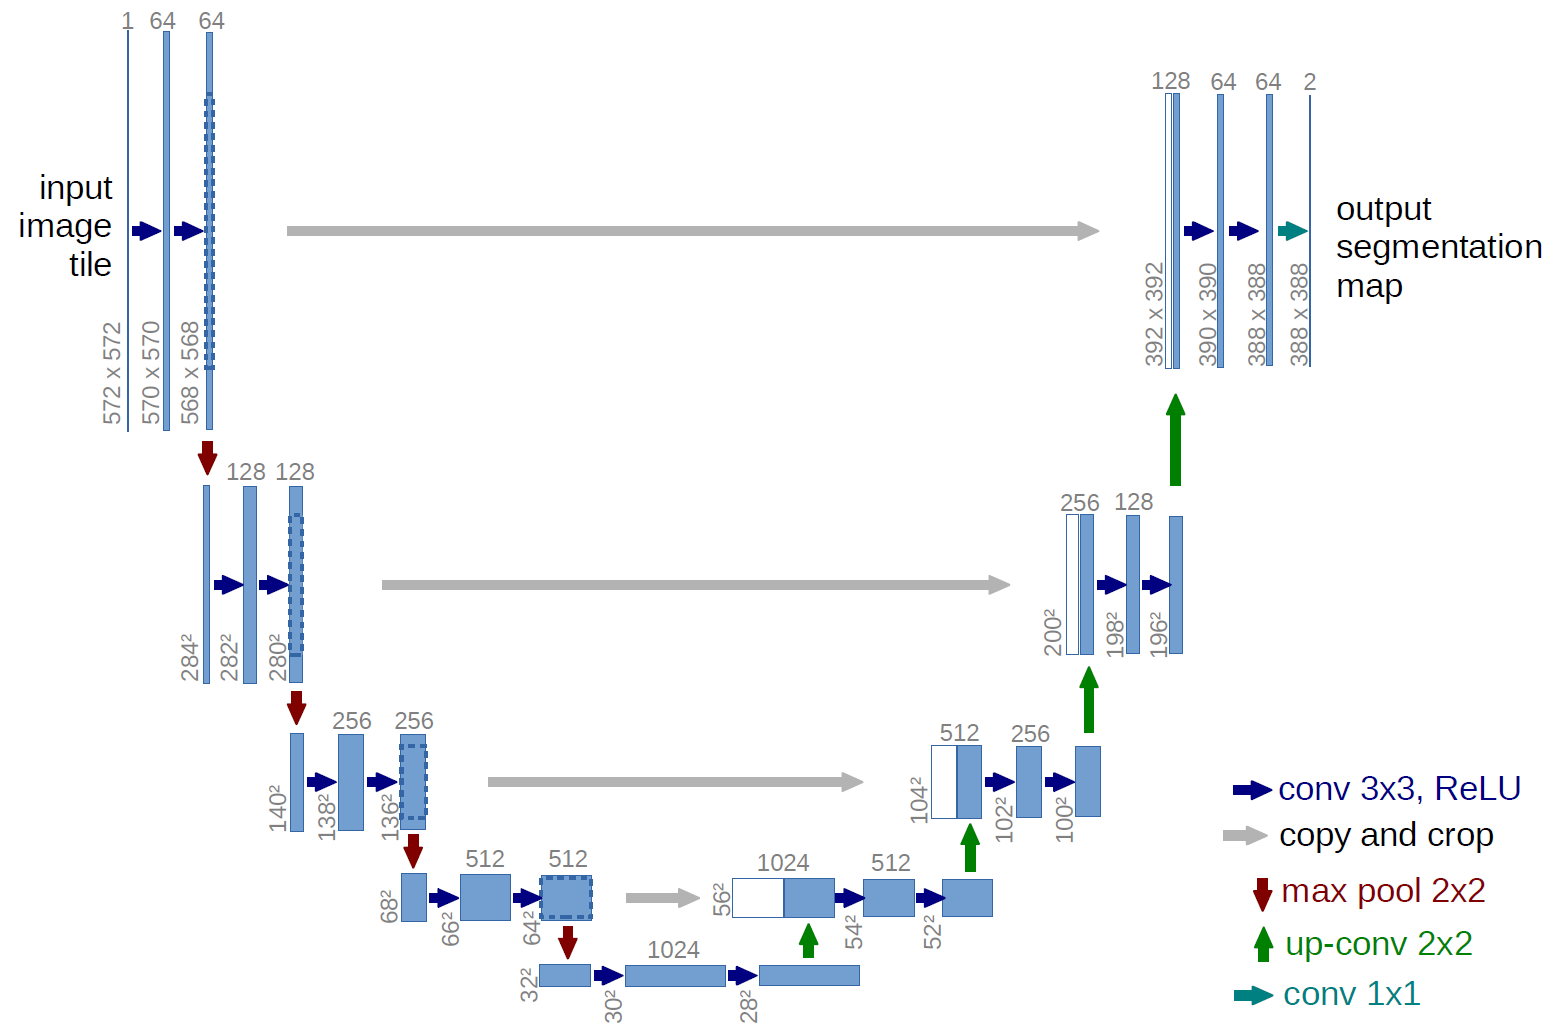
\includegraphics[width=0.75\textwidth]{u-net-architecture.png}
        \caption{U-Net Architecture, blue boxes are feature maps and white boxes are copied feature maps (\cite{ronneberger2015unet})}
        \label{fig_unet}
    \end{figure}